\section{Previous Work} \label{sec:previous_work}
A first version of PowerPedia already exists. It was implemented as part of Adrian Merkle's Master thesis~\cite{merklepp}. This prototype was realized as an extension to the eMeter system, which is described further thereafter.
In order to demonstrate the functionality of Powerpedia, Adrian Merkle also implemented an Android eMeter application based on the already existing iPhone application. This mobile phone application serves as a user interface to access the platform.

\subsection{Overview}
\begin{center}
\begin{figure}
 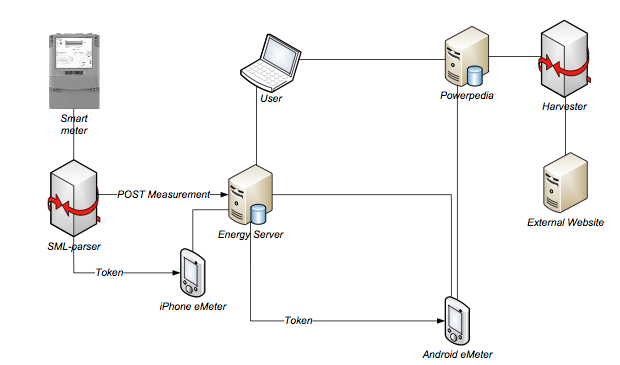
\includegraphics[width=15cm]{Images/emeter_overview.png}
 \label{emeter_overview}
 \caption{Overview over the complete system}
\end{figure}
\end{center}
\todo{replace figure}
Figure~\ref{emeter_overview} depicts a complete overview of the current status of the system. In the original implementation of the eMeter system, there were only the smart meter, SML-parser, Energy Server, User, and iPhone eMeter components.

The SML-parser polls the smart meter to get the current electricity consumption value and pushes it to the Energy Server. It also broadcasts the unique identifier (token) of the smart meter, which can be picked up by the iPhone eMeter client to add the corresponding smart meter to the list of accessible smart meters. For the Android application, this token can be found on the Energy Server. Both mobile phone applications communicate with the Energy Server to get measurement data. The Android version also interacts with PowerPedia. PowerPedia uses the harvester module for data initialization, which gets the corresponding data from external websites. 
PowerPedia and the Energy Server both have a web interface that is accessible by users.  

\subsection{eMeter System}
The eMeter system is an interactive energy consumption monitoring system. It allows users to track the energy usage on a household and device level. By providing instantaneous feedback on the overall energy usage and letting user interactively measure and compare the consumption of individual devices, the system helps to identify where energy is wasted and decrease the overall energy consumption.  

The system builds upon \textit{smart electricity meters}\footnote{e.g Landis+Gyr ZMK410 smart meter, as used in the system}, which allow to monitor the consumption in real or near-real time. Data is recorded in regular intervals. Also, compared to regular meters, smart meters have a communication interface intended for remote reading for billing purposes. There is quite a number of households with smart electricity meters already and this number will be increasing even more\footnote{For example, energy monitoring systems are required for newly build or renovated houses in Europe by law\cite{eu_meter}}, so the system achieves a low usage barrier. No setup or installation is 

eMeter combines smart electricity meters with a mobile phone application, which makes the system very easy to use.  All the user has to do is downloading the application for the mobile phone over the internet.

The system was first designed and implemented in a bachelor thesis~\cite{roediger}. 

\subsubsection{eMeter Architecture}\label{sec:emeter_architecture}
\missingfigure{eMeter architecture}
The eMeter extends the functionality of the smart electricity meter and consists of three components. The first component, a SML parser communicates directly with the meter. The second component, the Energy Server makes the measurement available using URLs. Last, a portable user interface allows users to get real-time feedback from the Energy Server and lets users measure and display current consumption data.

\minisec{SML parser}
The smart electricity meter measures the total energy consumption that results from devices attached to the electric circuit of the household. Those measurements are polled by the Smart Message Language (SML)\footnote{The SML specification of the SyM$^2$ can be found here: \url{http://www.vde.com/de/fnn/extras/Sym2/Infomaterial/Documents/SML_081112_103.pd}} parser, which is connected to the meter via a LAN-cable. Its task is to read the binary encoded message. Then, it  forwards a relevant subset of the data to the Energy Server as a HTTP message, encoded as a JSON string. \todo{what are the meanings of the values that are transmitted? E.g what are the three phases?}

\minisec{Energy Server}
The Energy Server is the central instance that stores and manages the measurements from the SML-parser. By having a server between the SML parser and the user interface, clients can access the data using the HTTP protocol. The server also has a web user interface. Statistical information such as total measured energy in kWh or smart meters attached to the system, all the measurements received from the parser and other data can be accessed via this interface. 

\minisec{Mobile Phone Application}
\begin{center}
\begin{figure}
 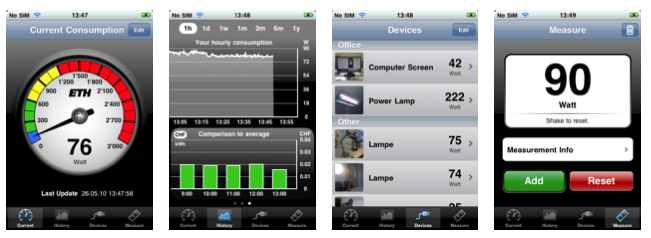
\includegraphics[width=16cm]{Images/iphone_screens.png}
 \label{iphone_screens}
 \caption{Mobile application user interface}
\end{figure}
\end{center}
\todo{Replace image}
In order to motivate users to use the eMeter system over a long-time period, an attractive, easy accessible mobile phone user interface was created. This application is the front-end of the system. It communicates with the Energy Server to get electricity usage data.
With this data, the current electricity consumption is visualized in real-time and historical usage is calculated. It also allows users to interactively measure the energy consumption of a single or multiple domestic appliances. 

There are four different views as displayed in figure~\ref{iphone_screens}:

\begin{description}
 \item[Overview] The overview screen shows the current consumption of the household, visualized with the help of a gauge. There are four different colors to help users to classify their current consumption and to compare it to historical consumption. The gauge is self-learning, it adapts the colors and ranges according the consumption. The blue range is the base load.
 \item[History] The history view displays the historic consumption as stored on the Energy Server in a load curve. Statistical information such as cumulative or average, minimum or maximum consumption can be found here as well.
 \item[Measure] In this view, users can interactively measure the consumption or standby usage of a device by clicking on the start button and thereafter turning the device on or off. The result in Watt is displayed right away. The measured device can be stored in the device list of the application that stores all the devices that have been measured. Further information such as picture, location or utilization can be specified.
 \item[Devices] The devices screen shows all the previously created devices. They can be sorted according to their location or energy usage to find the biggest energy guzzlers right away.   
\end{description}
Originally, the mobile phone application was developed in Objective-C for the iPhone.

\subsection{PowerPedia Prototype}
The PowerPedia prototype is a web platform which serves as a central server for consumption measurement data created by users with the eMeter system. The prototype was build as an independent module of the eMeter system to enhance its features, namely putting electricity consumption values in a larger context beyond mere numbers.

PowerPedia was developed as a means to make the energy consumption more transparent for users~\cite{merklepp}. The main objective of the system was to "allow users to better access their electricity consumption and energy efficiency of their appliances"~\cite{weiss:inprocPUC:2012}. To achieve this goal, the PowerPedia prototype is centered around the idea of action guided feedback. It offers the possibility to compare the energy consumption of household appliances to the consumption of devices that reside in the same device category~\cite{merklepp}. User can upload their measurements made with the eMeter system and get immediate feedback. To help users conserve energy, PowerPedia also provides specific tips on how to be more energy efficient.

\subsubsection{Android eMeter Client}
In order to demonstrate the functionality of PowerPedia, a second version of the mobile phone application was developed. This application was realized as an Android application and is based on the one for the iPhone (as described in~\ref{sec:emeter_architecture}). Is used as a user interface to access the platform.

A detailed analysis of the functionality and technical realization of both the web platform and mobile phone application follows in~\ref{sec:prototype_analysis}.